% !Mode:: "TeX:UTF-8"

\chapter{分层的动态温度管理方法}\label{sec:new_method}

在这一章,针对高性能众核微处理器,提出了新的分层动态温度管理方法。新方法是基于模型预测控制而且采用了任务迁移和DVFS。

众核处理器上执行结合任务迁移的MPC是一个挑战,因为但处理器处理器核数非常的大,
用复杂度为$O(n^{3})$的匈牙利算法计算任务迁移的决策需要花费大量的时间,这个时间可以看成是二部图匹配的时间。
为了扩展到具有大量处理器核的众核处理器,新的方法将处理器分成块,在两个层次上进行任务迁移决策:块内(低层)和块间(高层)。
首先在低层,也就是块内执行当前功耗和期望功耗组成的二部图匹配。在低层内没有匹配上的功耗元素,收集起来形成高层,也就是块间。
在高层,用改进的迭代最小割算法将高层分成“优化”块,在每个“优化”块执行二部图匹配。
高层最后没有匹配的功耗元素用DVFS来处理,以保证绝对的温度安全。
分层算法通过减小二部图匹配规模来降低计算开销,而且匹配是并行执行的,大大减少了计算时间,所以该算法可以扩展到众核系统。

\section{低层块内任务迁移}\label{sec:parts}

首先,我们将众核处理器分割成块。作为第一步,我们可以简单根据核的位置分割处理器。
就是在空间上直接划分处理器成块。
这一步分割不需要任何开销。我们通常将方形的块叫普通块,在边缘可能会出现矩形或者小的方形块,把这些称作边缘块。

块内匹配就是执行\ref{sec:dtm_mpc} 节中说明了二部图匹配的过程,这个叫做低层匹配。对每一个块,指定一个块内的核执行匹配的计算。
从整个芯片来看,低层匹配的计算是并行执行的。所以底层匹配引入的延迟时间只是一个普通块低层匹配的时间(注意,边缘块比常规快要小,也就是说它们的计算时间也并不计算在内)。

可以调整块内的核数以实现整个算法更小的延迟时间:如果核数很大,低层的功耗匹配将会占用更多的时间,
但是可以发现更多的匹配对,将会剩余更少的未匹配功耗到高层,这样高层匹配处理时间就会减少。

图~\ref{fig:cpu_partition} (a)是一个简单的低层划分的例子。这是一个100核微处理器,被划分为四个16核普通块(标记为A、B、D、E),五个核数4到8核的边缘块(标记为C、F、G、H、I)。
低层的功耗匹配将在每一个块内执行。图~\ref{fig:bi2} 展示的正是图~\ref{fig:cpu_partition} (a)中块I内的二部图匹配。

\begin{figure}[H]
  \centering
    \subfigure[微处理器分割成块准备进行低层二部图匹配。]
  {
    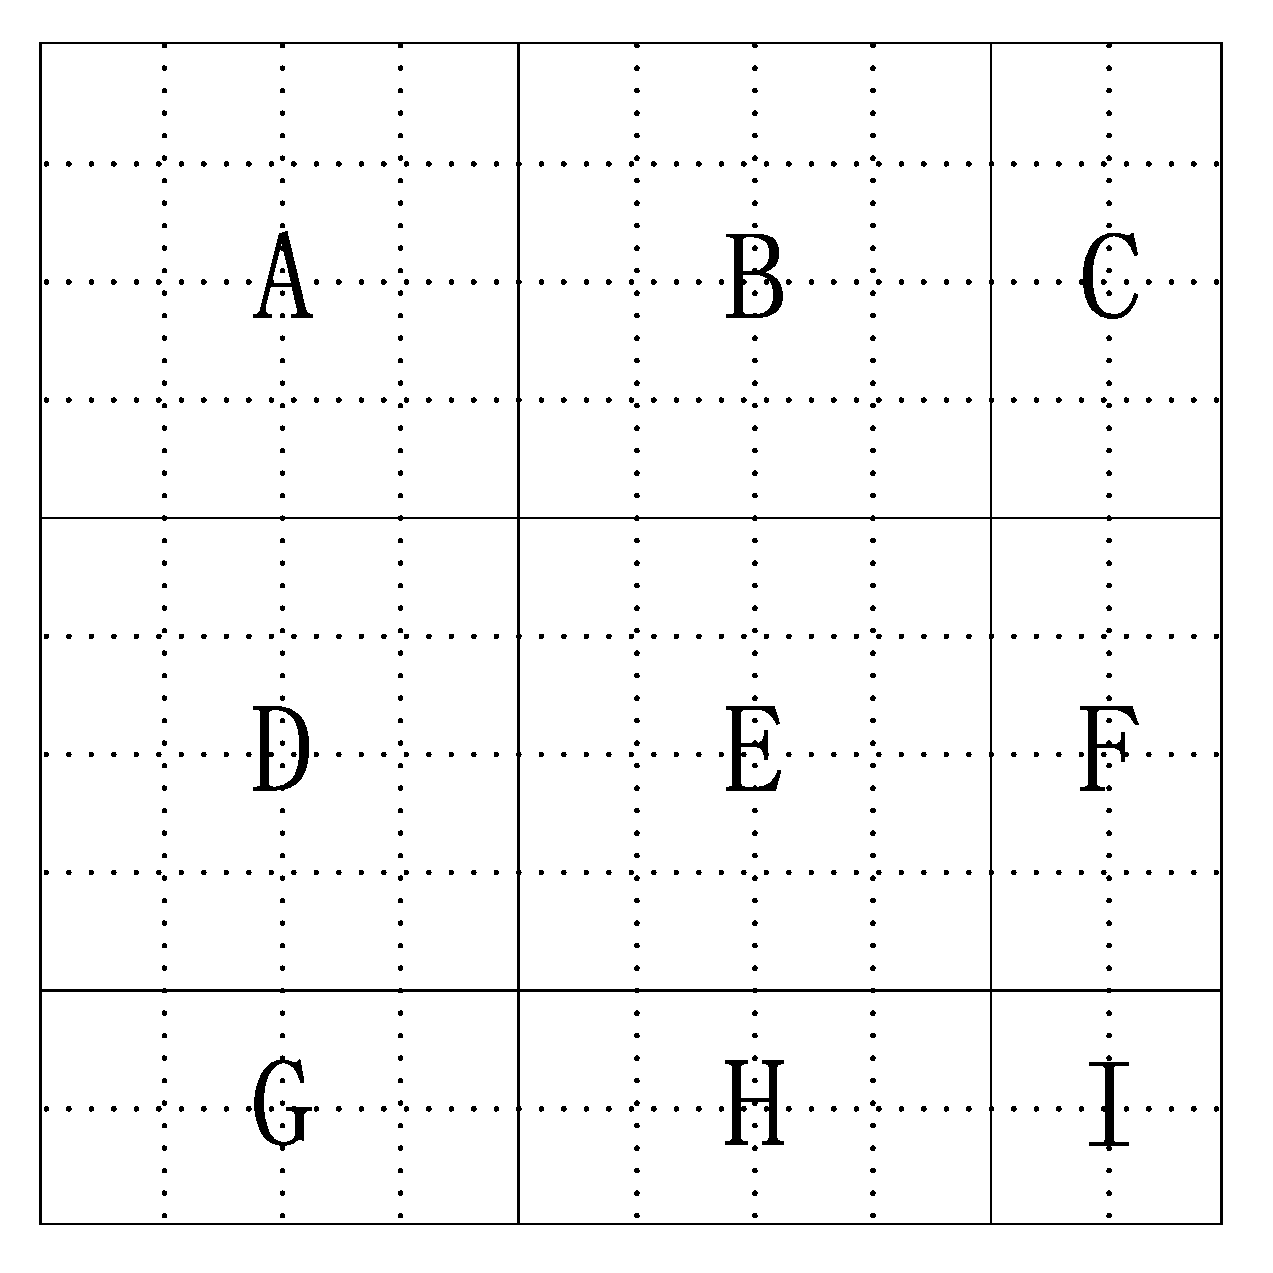
\includegraphics[width=0.32\columnwidth]{fig/part1}
  }
  \subfigure[低层二部图匹配之后留下的未匹配核(红色)。]
  {
    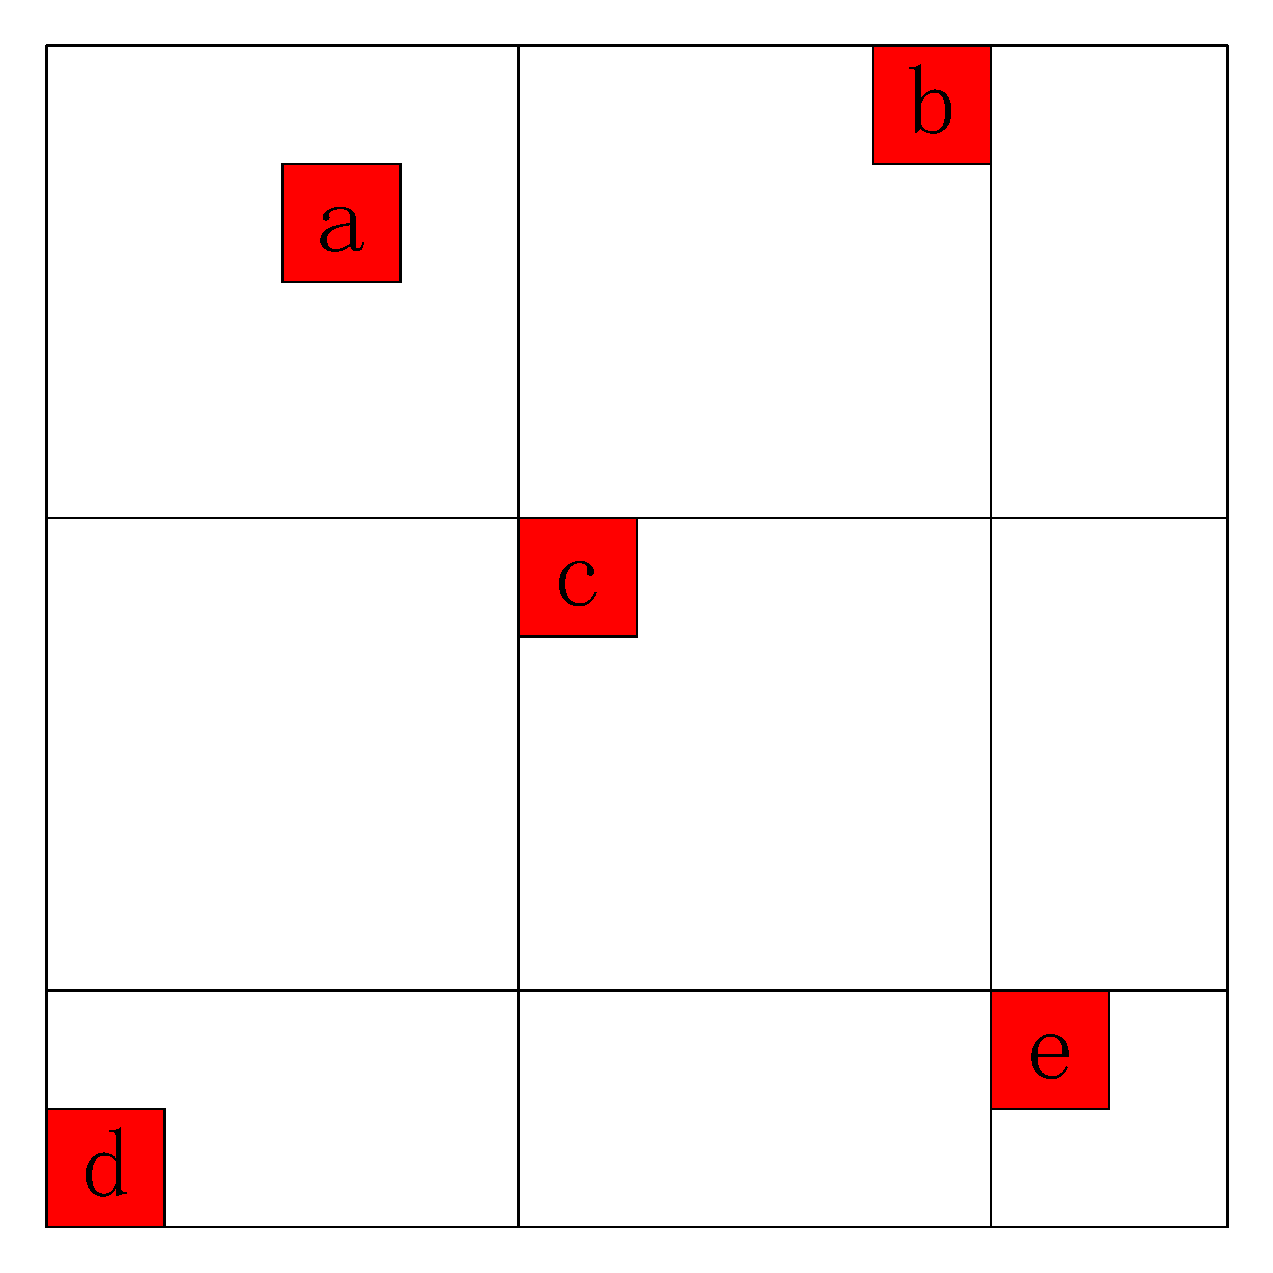
\includegraphics[width=0.32\columnwidth]{fig/partmod}
  }
  \caption{100核微处理器的垂直视图 (作为分层算法的一个例子)。}\label{fig:cpu_partition}
\end{figure}

显然,只执行低层的块内功耗匹配不足以找到所有的匹配对。
例如,在图~\ref{fig:cpu_partition} (a)的块 I 中, 图~\ref{fig:bi2} (b) 已经表示出
功耗 $p_1$ 和 $\bar{p}_4$ 不能匹配。
对低层匹配阶段块内未匹配功耗直接执行DVFS并不是好办法,因为一个块内的未匹配功耗可能在其他块找到很好匹配的期望功耗。
这样就可以避免太多不必要的DVFS行为,将性能损失最小化。
所以,我们可以收集所有块内低层匹配时未匹配的功耗,形成高层。图~\ref{fig:cpu_partition} (b)中表示出第一次底层匹配后未匹配的功耗。

\section{高层块间任务迁移}\label{sec:fm}
























































